% Figure 5: Macro-Micro Bidirectional Causation
% Showing downward and upward causation in the VFD-Orch framework
\documentclass[tikz,border=5pt]{standalone}
\usepackage{tikz}
\usetikzlibrary{calc,decorations.pathmorphing,arrows.meta,shapes.geometric,positioning,patterns}

\begin{document}
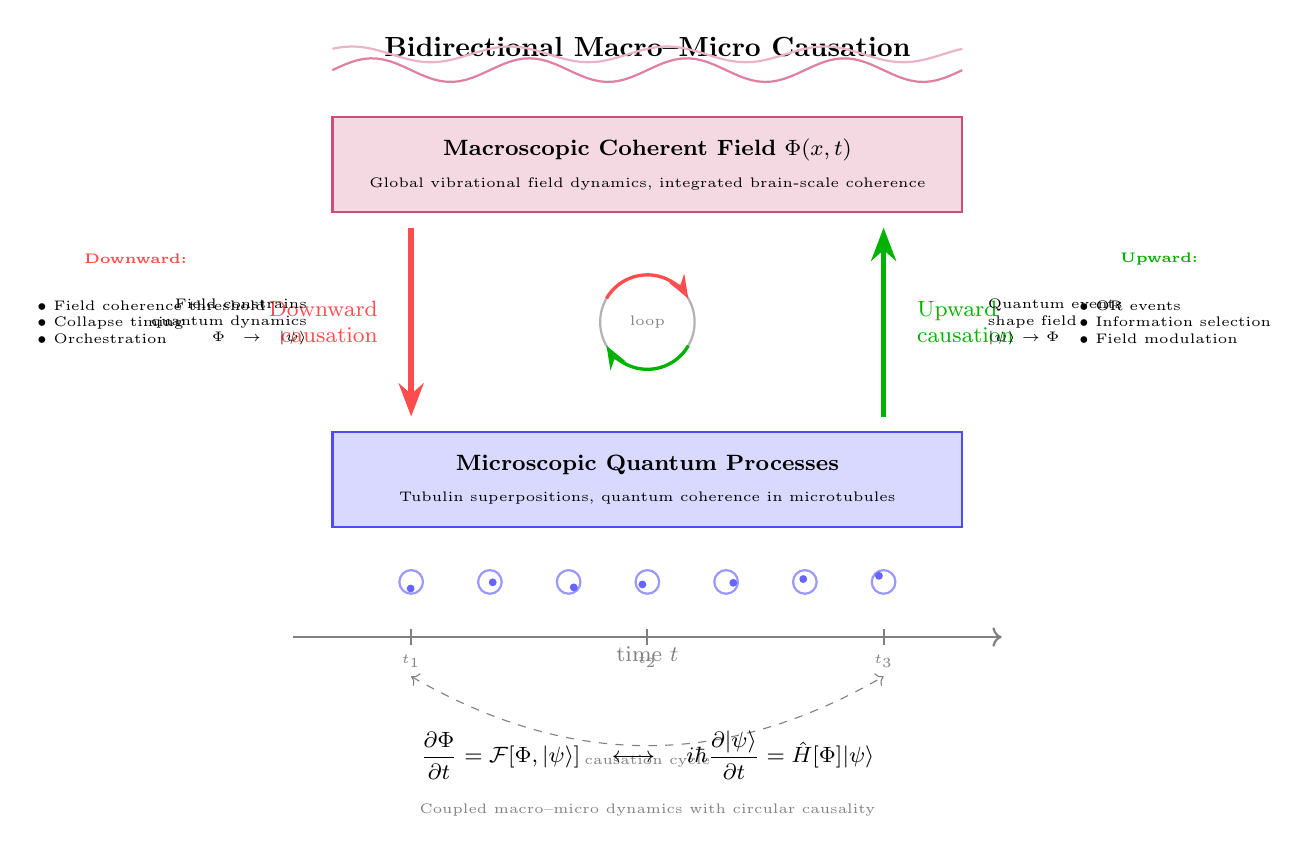
\begin{tikzpicture}[scale=1,
    level/.style={rectangle,draw,thick,minimum width=8cm,minimum height=1.2cm,align=center,font=\footnotesize},
    arrow/.style={->,very thick,>=Stealth}
]

% === Title ===
\node[font=\bfseries] at (0,5.5) {Bidirectional Macro--Micro Causation};

% === MACRO LEVEL (Top) ===
\node[level,fill=purple!15,draw=purple!70] (macro) at (0,4) {
    \textbf{Macroscopic Coherent Field} $\Phi(x,t)$\\[2pt]
    {\tiny Global vibrational field dynamics, integrated brain-scale coherence}
};

% Field visualization above macro
\draw[purple!50,thick,domain=-4:4,samples=100] plot (\x,{5.2+0.15*sin(180*\x)});
\draw[purple!30,thick,domain=-4:4,samples=100] plot (\x,{5.4+0.1*sin(180*\x+45)});

% === MICRO LEVEL (Bottom) ===
\node[level,fill=blue!15,draw=blue!70] (micro) at (0,0) {
    \textbf{Microscopic Quantum Processes}\\[2pt]
    {\tiny Tubulin superpositions, quantum coherence in microtubules}
};

% Quantum visualization below micro
\foreach \x in {-3,-2,-1,0,1,2,3} {
    \draw[blue!40,thick] (\x,-1.3) circle (0.15);
    \fill[blue!60] (\x,-1.3) ++(rand*0.1,rand*0.1) circle (0.05);
}

% === DOWNWARD CAUSATION (Left arrow) ===
\draw[arrow,red!70,line width=2pt] (-3,3.2) -- (-3,0.8);
\node[left,font=\footnotesize,red!70,align=right] at (-3.3,2) {Downward\\causation};

% Annotation for downward
\node[left,font=\tiny,text width=2.2cm,align=right] at (-4.2,2) {
    Field constrains\\
    quantum dynamics\\
    $\Phi \to |\psi\rangle$
};

% === UPWARD CAUSATION (Right arrow) ===
\draw[arrow,green!70!black,line width=2pt] (3,0.8) -- (3,3.2);
\node[right,font=\footnotesize,green!70!black,align=left] at (3.3,2) {Upward\\causation};

% Annotation for upward
\node[right,font=\tiny,text width=2.2cm,align=left] at (4.2,2) {
    Quantum events\\
    shape field\\
    $|\psi\rangle \to \Phi$
};

% === CIRCULAR CAUSALITY SYMBOL ===
\begin{scope}[shift={(0,2)}]
    \draw[thick,gray!60] (0,0) circle (0.6);
    \draw[arrow,red!70] (150:0.6) arc (150:30:0.6);
    \draw[arrow,green!70!black] (-30:0.6) arc (-30:-150:0.6);
    \node[font=\tiny,gray] at (0,0) {loop};
\end{scope}

% === MEDIATING PROCESSES (Middle) ===
\node[font=\tiny,gray,align=center] at (0,2) {};

% Left side details
\begin{scope}[shift={(-6.5,2)}]
    \node[font=\tiny\bfseries,red!70] at (0,0.8) {Downward:};
    \node[font=\tiny,align=left] at (0.2,0) {
        $\bullet$ Field coherence threshold\\
        $\bullet$ Collapse timing\\
        $\bullet$ Orchestration
    };
\end{scope}

% Right side details
\begin{scope}[shift={(6.5,2)}]
    \node[font=\tiny\bfseries,green!70!black] at (0,0.8) {Upward:};
    \node[font=\tiny,align=left] at (0.2,0) {
        $\bullet$ OR events\\
        $\bullet$ Information selection\\
        $\bullet$ Field modulation
    };
\end{scope}

% === TIME EVOLUTION ===
\draw[->,thick,gray] (-4.5,-2) -- (4.5,-2);
\node[below,font=\footnotesize,gray] at (0,-2) {time $t$};

% Time markers showing causation cycle
\foreach \t/\label in {-3/$t_1$, 0/$t_2$, 3/$t_3$} {
    \draw[gray,thick] (\t,-1.9) -- (\t,-2.1);
    \node[below,font=\tiny,gray] at (\t,-2.1) {\label};
}

% Cycle annotation
\draw[<->,gray,dashed] (-3,-2.5) to[bend right=30] node[below,font=\tiny] {causation cycle} (3,-2.5);

% === Bottom equation ===
\node[font=\footnotesize] at (0,-3.5) {
    $\displaystyle \frac{\partial \Phi}{\partial t} = \mathcal{F}[\Phi, |\psi\rangle]$
    \quad $\longleftrightarrow$ \quad
    $\displaystyle i\hbar\frac{\partial |\psi\rangle}{\partial t} = \hat{H}[\Phi]|\psi\rangle$
};

\node[font=\tiny,gray] at (0,-4.2) {Coupled macro--micro dynamics with circular causality};

\end{tikzpicture}
\end{document}
